\begin{center}
	\begin{tabular}{M{9.25cm}M{8.75cm}}
		\textbf{TRƯỜNG THCS-THPT NGUYỄN KHUYẾN}& \textbf{ÔN TẬP KIỂM TRA CUỐI HỌC KÌ I}\\
		\textbf{MÃ ĐỀ: 001}& \textbf{Bài thi môn: VẬT LÝ 10}\\
		\textit{(Đề thi có 04 trang)}& \textit{Thời gian làm bài: 45 phút, không kể phát đề}
		
		\noindent\rule{4cm}{0.8pt} \\
	\end{tabular}
\end{center}
\setcounter{section}{0}
\section{Câu trắc nghiệm nhiều phương án lựa chọn}
\textit{Thí sinh trả lời từ câu 1 đến câu 18. Mỗi câu hỏi thí sinh chọn một phương án}
\setcounter{ex}{0}
\Opensolutionfile{ans}[ans/D10-CK1-001-TN]

% ===================================================================
\begin{ex}
	Đại lượng đặc trưng cho mức quán tính của một vật là
	\choice
	{vận tốc của vật}
	{\True khối lượng của vật}
	{kích thước của vật}
	{gia tốc của vật}
	\loigiai{}
\end{ex}
% ===================================================================
\begin{ex}
	Gia tốc rơi tự do phụ thuộc vào yếu tố nào?
	\choice
	{Quãng đường vật đi được}
	{\True Vĩ độ địa lí và độ cao}
	{Vĩ độ địa lí}
	{Độ cao}
	\loigiai{}
\end{ex}
% ===================================================================
\begin{ex}
	Lực căng dây \textbf{không có} đặc điểm nào sau đây?
	\choice
	{\True Độ lớn luôn bằng trọng lượng của vật}
	{Phương trùng với phương sợi dây}
	{Điểm đặt ở hai đầu dây, chỗ tiếp xúc với vật}
	{Chiều luôn hướng vào giữa sợi dây}
	\loigiai{}
\end{ex}
% ===================================================================
\begin{ex}
	Trong chuyển động thẳng biến đổi đều, đại lượng không đổi theo thời gian là
	\choice
	{tọa độ}
	{quãng đường}
	{vận tốc}
	{\True gia tốc}
	\loigiai{}
\end{ex}

% ===================================================================
\begin{ex}
	Câu nào sau đây là đúng khi nói về lực hấp dẫn do Trái Đất tác dụng lên Mặt Trăng và do Mặt Trăng tác dụng lên Trái Đất?
	\choice
	{Hai lực này cùng phương cùng chiều}
	{\True Hai lực này cùng phương ngược chiều}
	{Hai lực này cùng chiều, cùng độ lớn}
	{Phương của hai lực này không thay đổi và luôn trùng nhau}
	\loigiai{}
\end{ex}
% ===================================================================
\begin{ex}
	Một vật chuyển động thẳng đều khi
	\choice
	{hợp lực tác dụng vào nó cùng chiều chuyển động}
	{\True các lực tác dụng vào nó cân bằng nhau}
	{hợp lực tác dụng vào nó không đổi}
	{hợp lực tác dụng vào nó ngược chiều chuyển động}
	\loigiai{}
\end{ex}
% ===================================================================
\begin{ex}
	Hệ số ma sát giữa hai mặt tiếp xúc sẽ thay đổi như thế nào nếu lực ép hai mặt đó tăng lên?
	\choice
	{Tăng lên}
	{Giảm đi}
	{\True Không thay đổi}
	{Còn phụ thuộc vào diện tích hai bề mặt}
	\loigiai{}
\end{ex}
% ===================================================================
\begin{ex}
	\immini{Trên hình bên là đồ thị tọa độ - thời gian của một vật chuyển động thẳng. Hãy cho biết thông tin nào sau đây là \textbf{sai}?
		\choice
		{Tọa độ ban đầu của vật là $x_0=\SI{10}{\meter}$}
		{\True Trong $\SI{5}{\second}$ đầu tiên, vật đi được $\SI{25}{\meter}$}
		{Vật chuyển động theo chiều dương của trục tọa độ}
		{Gốc thời gian được chọn là thời điểm vật ở cách gốc tọa độ $\SI{10}{\meter}$}}
		{
		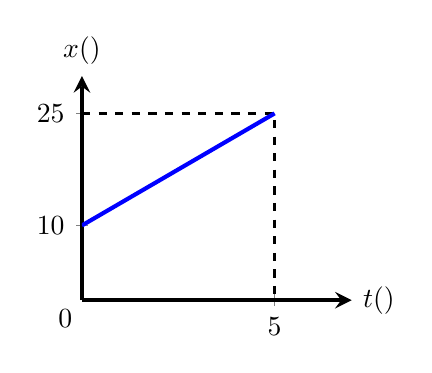
\begin{tikzpicture}  
			\begin{axis}[  ultra thick,
				xmin=0,  
				xmax=7,  
				xtick={0,5},
				ytick={0,10,25},
				ymin=0,  
				ymax=30, 
				samples=300,
				axis lines=center, 
				xlabel=$\xsi{t}{\left(\si{\second}\right)}$, 		ylabel=$\xsi{x}{\left(\si{\meter}\right)}$,
				every axis y label/.style={at=(current axis.above origin),anchor=south},  
				every axis x label/.style={at=(current axis.right of origin),anchor=west},  scale=0.5]
				\draw[line width=1pt, dashed] (axis cs: 0,25)--(axis cs: 5,25)--(axis cs: 5,0);
				\addplot [line width=1.5pt, blue, smooth, domain=0:5] {10+3*x};  
				\coordinate (O) at (axis cs: 0,0);
			\end{axis}  
			\node[below left] at (O) {0};
		\end{tikzpicture}
		}
	\loigiai{}
\end{ex}
% ===================================================================
\begin{ex}
Một đoàn tàu rời ga chuyển động thẳng nhanh dần, sau 1 phút đạt vận tốc $\SI{40}{\kilo\meter/\hour}$. Gia tốc trung bình của đoàn tàu gần giá trị nào sau đây nhất?	
	\choice
	{$\SI{0.188}{\meter/\second^2}$}
	{$\SI{0.288}{\meter/\second^2}$}
	{$\SI{0.285}{\meter/\second^2}$}
	{\True $\SI{0.185}{\meter/\second^2}$}
	\loigiai{}
\end{ex}
% ===================================================================
\begin{ex}
	Hình vẽ nào sau đây biểu diễn đúng lực tổng hợp $\vec{F}$ của hai lực $\vec{F}_1$ và $\vec{F}_2$?
	\choice
	{\begin{tikzpicture}
			\coordinate (A) at (0,0);
			\coordinate (B) at ($(A)+(2.5,0)$);
			\coordinate (C) at ($(B)+(90:1.5)$);
			\draw[blue, line width=1.5pt, -stealth] (A)--(B);
			\draw[blue, line width=1.5pt, -stealth] (B)--(C);
			\draw[blue, line width=1.5pt, -stealth] (A)--(C);
			\node[below, blue] at ($(A)!0.5!(B)$) {$\vec{F}$};
			\node[right, blue] at ($(B)!0.5!(C)$) {$\vec{F}_2$};
			\node[above left, blue] at ($(A)!0.5!(C)$) {$\vec{F}_1$};
	\end{tikzpicture}}
	{\begin{tikzpicture}
			\coordinate (O) at (0,0);
			\coordinate (A) at (2,0);
			\coordinate (C) at ($(A)+(-60:1.5)$);
			\coordinate (B) at ($(O)+(-60:1.5)$);
			\draw[dashed, line width=1pt] (A)--(C)--(B);
			\draw[-stealth, blue, line width=1.5pt] (O)--(A);
			\draw[-stealth, blue, line width=1.5pt] (O)--(B);
			\draw[-stealth, blue, line width=1.5pt] (O)--(C);
			\node[below left, blue] at ($(O)!0.5!(B)$) {$\vec{F}$};
			\node[above, blue] at ($(O)!0.5!(A)$) {$\vec{F}_1$};
			\node[below, blue] at ($(O)!0.5!(C)$) {$\vec{F}_2$};
	\end{tikzpicture}}
	{\True \begin{tikzpicture}
			\coordinate (O) at (0,0);
			\coordinate (A) at ($(O)+(90:2.5)$);
			\coordinate (B) at ($(O)+(180:2)$);
			\coordinate (C) at ($(A)+(180:2)$);
			\draw[dashed, line width=1pt] (A)--(C)--(B);
			\draw[blue, line width=1.5pt, -stealth] (O)--(A);
			\draw[blue, line width=1.5pt, -stealth] (O)--(C);
			\draw[blue, line width=1.5pt, -stealth] (O)--(B);
			\node[above right, blue] at ($(O)!0.5!(C)$) {$\vec{F}$};
			\node[above, blue] at ($(O)!0.5!(B)$) {$\vec{F}_2$};
			\node[right, blue] at ($(O)!0.5!(A)$) {$\vec{F}_1$};
	\end{tikzpicture}}
	{\begin{tikzpicture}
			\coordinate (O) at (0,0);
			\coordinate (A) at ($(O)+(2,0)$);
			\coordinate (B) at ($(O)+(60:2)$);
			\draw[blue, -stealth, line width=1.5pt] (O)--(A);
			\draw[blue, -stealth, line width=1.5pt] (O)--(B);
			\draw[blue, -stealth, line width=1.5pt] (A)--(B);
			\node[above, blue] at ($(O)!0.5!(A)$) {$\vec{F}_2$};
			\node[right, blue] at ($(A)!0.5!(B)$) {$\vec{F}$};
			\node[left, blue] at ($(O)!0.5!(B)$) {$\vec{F}_1$};
	\end{tikzpicture}}
	\loigiai{}
\end{ex}
% ===================================================================
\begin{ex}
\immini{Một vật chuyển động thẳng có đồ thị vận tốc - thời gian như hình bên. Tính chất chuyển động của vật là	
	\choice
	{Chuyển động chậm dần đều theo chiều dương rồi nhanh dần đều theo chiều âm}
	{Chuyển động nhanh dần đều theo chiều dương rồi chậm dần đều theo chiều âm}
	{\True Chuyển động nhanh dần đều rồi chậm dần đều theo chiều dương}
	{Chuyển động nhanh dần đều rồi chậm dần đều theo chiều âm}}
	{
	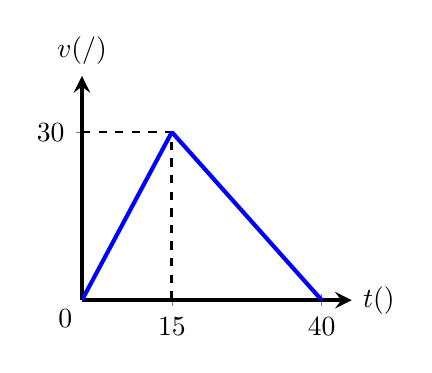
\begin{tikzpicture}  
		\begin{axis}[  ultra thick,
			xmin=0,  
			xmax=45,  
			xtick={0,15,40},
			ytick={0,30},
			ymin=0,  
			ymax=40, 
			samples=300,
			axis lines=center, 
			xlabel=$\xsi{t}{\left(\si{\second}\right)}$, 		ylabel=$\xsi{v}{\left(\si{\meter/\second}\right)}$,
			every axis y label/.style={at=(current axis.above origin),anchor=south},  
			every axis x label/.style={at=(current axis.right of origin),anchor=west},  scale=0.5]
			\draw[line width=1pt, dashed] (axis cs: 0,30)--(axis cs: 15,30)--(axis cs: 15,0);
			\addplot [line width=1.5pt, blue, smooth, domain=0:15] {2*x};  
			\addplot [line width=1.5pt, blue, smooth, domain=15:40] {30-1.2*(x-15)}; 
			\coordinate (O) at (axis cs: 0,0);
		\end{axis}  
		\node[below left] at (O) {0};
	\end{tikzpicture}
	}
	\loigiai{}
\end{ex}
% ===================================================================
\begin{ex}
	Một lực không đổi tác dụng vào một vật có khối lượng $\SI{5.0}{\kilogram}$ làm vận tốc của nó tăng dần từ $\SI{2.0}{\meter}$ đến $\SI{8.0}{\meter/\second}$ trong $\SI{3.0}{\second}$. Độ lớn lực tác dụng vào vật là
	\choice
	{\True $\SI{10}{\newton}$}
	{$\SI{5}{\newton}$}
	{$\SI{15}{\newton}$}
	{$\SI{1}{\newton}$}
	\loigiai{}
\end{ex}
% ===================================================================
\begin{ex}
Cho biết khối lượng của Trái Đất là $M=\SI{6E24}{\kilogram}$; khối lượng của một hòn đá $m=\SI{2.3}{\kilogram}$; gia tốc trọng trường là $g=\SI{9.81}{\meter/\second^2}$. Hòn đá hút Trái Đất một lực có độ lớn xấp xỉ
	\choice
	{$\SI{15.82}{\newton}$}
	{$\SI{20.24}{\newton}$}
	{\True $\SI{22.56}{\newton}$}
	{$\SI{32}{\newton}$}
	\loigiai{}
\end{ex}
% ===================================================================
\begin{ex}
	Một dòng sông rộng $\SI{100}{\meter}$ và dòng nước chảy với vận tốc $\SI{3}{\meter/\second}$ so với bờ. Một chiếc thuyền đi ngang sông với vận tốc $\SI{4}{\meter/\second}$ so với dòng nước. Quãng đường mà thuyền đi được khi sang đến bờ bên kia là
	\choice
	{$\SI{150}{\meter}$}
	{\True $\SI{125}{\meter}$}
	{$\SI{100}{\meter}$}
	{$\SI{50}{\meter}$}
	\loigiai{}
\end{ex}
% ===================================================================
\begin{ex}
	Một vật có khối lượng $\SI{70}{\kilogram}$ chuyển động thẳng đều trên mặt sàn nằm ngang dưới tác dụng của lực kéo không đổi và có độ lớn $\SI{210}{\newton}$ theo phương ngang. Lấy $g=\SI{10}{\meter/\second^2}$. Hệ số ma sát trượt giữa vật và sàn là
	\choice
	{\True $0,3$}
	{$0,147$}
	{$3,3$}
	{$0,05$}
	\loigiai{}
\end{ex}
% ===================================================================
\begin{ex}
	Một vật khối lượng $\SI{2.5}{\kilogram}$ rơi thẳng đứng từ độ cao $\SI{100}{\meter}$ không vận tốc đầu, sau $\SI{20}{\second}$ thì chạm đất. Lấy gia tốc trọng trường $g=\SI{10}{\meter/\second^2}$. Nếu coi lực cản không khí tác dụng lên vật trong quá trình rơi là không đổi thì độ lớn của lực cản là
	\choice
	{$\SI{20}{\newton}$}
	{$\SI{40}{\newton}$}
	{\True $\SI{23.75}{\newton}$}
	{$\SI{25}{\newton}$}
	\loigiai{}
\end{ex}
% ===================================================================
\begin{ex}
Một vật chuyển động nhanh dần đều không vận tốc đầu. Trong giây thứ nhất vật đi được đoạn đường $s_1=\SI{3}{\meter}$, trong giây thứ hai vật đi được quãng đường $s_2$ bằng	
	\choice
	{$\SI{6}{\meter}$}
	{$\SI{3}{\meter}$}
	{\True $\SI{9}{\meter}$}
	{$\SI{12}{\meter}$}
	\loigiai{}
\end{ex}
% ===================================================================
\begin{ex}
	Một quả bóng có khối lượng $\SI{300}{\gram}$ bay với vận tốc $\SI{72}{\kilo\meter/\hour}$ đến đập vuông góc vào một bức tường thẳng đứng rồi bật trở lại theo phương cũ với vận tốc $\SI{54}{\kilo\meter/\hour}$. Thời gian va chạm $\SI{0.14}{\second}$. Lực do tường tác dụng lên quả bóng có độ lớn là
	\choice
	{\True $\SI{75}{\newton}$}
	{$\SI{70}{\newton}$}
	{$\SI{85}{\newton}$}
	{$\SI{65}{\newton}$}
	\loigiai{}
\end{ex}
\Closesolutionfile{ans}
\section{Câu trắc nghiệm đúng/sai} 
\textit{Thí sinh trả lời từ câu 1 đến câu 4. Trong mỗi ý \textbf{a)}, \textbf{b)}, \textbf{c)}, \textbf{d)} ở mỗi câu, thí sinh chọn đúng hoặc sai}
\setcounter{ex}{0}\\
\Opensolutionfile{ans}[ans/D10-CK1-001-TF]
% ===================================================================
\begin{ex}
	Nhận định các phát biểu sau về vai trò của lực ma sát nghỉ.\\
	Lực ma sát nghỉ
	\choiceTF[t]
	{\True đóng vai trò là lực phát động trong trường hợp chuyển động của người đi bộ, xe đạp, ô tô, tàu hỏa, \dots}
	{\True giúp ta cầm, nắm các vật}
	{giúp xe chuyển động chậm lại khi hãm phanh}
	{\True đóng vai trò truyền chuyển động bằng dây curoa trong các máy móc, băng chuyền, \dots}
	\loigiai{}
\end{ex}
% ===================================================================
\begin{ex}
	\immini{Một quả khúc côn cầu có khối lượng $\SI{0.30}{\kilogram}$ đang nằm trên mặt băng cứng, hoàn toàn nhẵn nằm ngang, thì chịu tác dụng đồng thời của hai cú đánh như hình bên. Lực $\vec{F}_1$ do cú đánh thứ nhất có độ lớn $\SI{5.0}{\newton}$ làm với trục $x$ về phía dưới một góc $\SI{20}{\degree}$. Lực $\vec{F}_2$ do cú đánh thứ hai có độ lớn $\SI{8.0}{\newton}$ làm với trục $x$ về phía trên một góc $\SI{60}{\degree}$.} {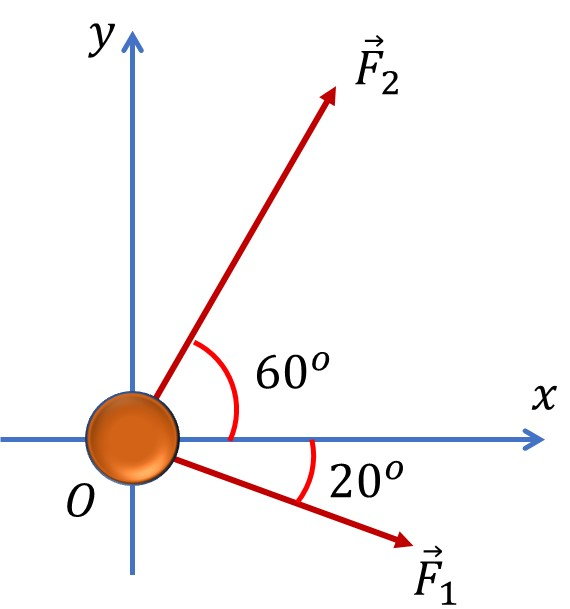
\includegraphics[scale=0.35]{figs/D10-CK1-002-2}}
	\choiceTF[t]
	{\True Hợp lực tác dụng lên quả khúc côn cầu có độ lớn $\SI{10.14}{\newton}$}
	{\True Sau cú đánh, quả khúc côn cầu chuyển động theo hướng hợp với trục $x$ góc $\SI{31}{\degree}$}
	{\True Trọng lực tác dụng lên quả khúc côn cầu không gây ra gia tốc cho nó}
	{\True Gia tốc của quả khúc côn cầu ngay sau cú đánh kép xấp xỉ $\SI{34}{\meter/\second^2}$}
	\loigiai{}
\end{ex}

% ===================================================================
\begin{ex}
\immini{	Huyền thoại điền kinh Usain Bolt người Jamaica đã lập kỉ lục thế giới ở nội dung chạy $\SI{100}{\meter}$ vào tháng 8/2009 tại Berlin. Usain Bolt đã hoàn thành cự li trên với thời gian $\SI{9.58}{\second}$. Ta giả sử rằng Bolt tăng tốc đều trong $\SI{3.00}{\second}$ đầu tiên để đạt tốc độ tối đa và duy trì tốc độ đó trong suốt phần còn lại của cuộc đua.}
{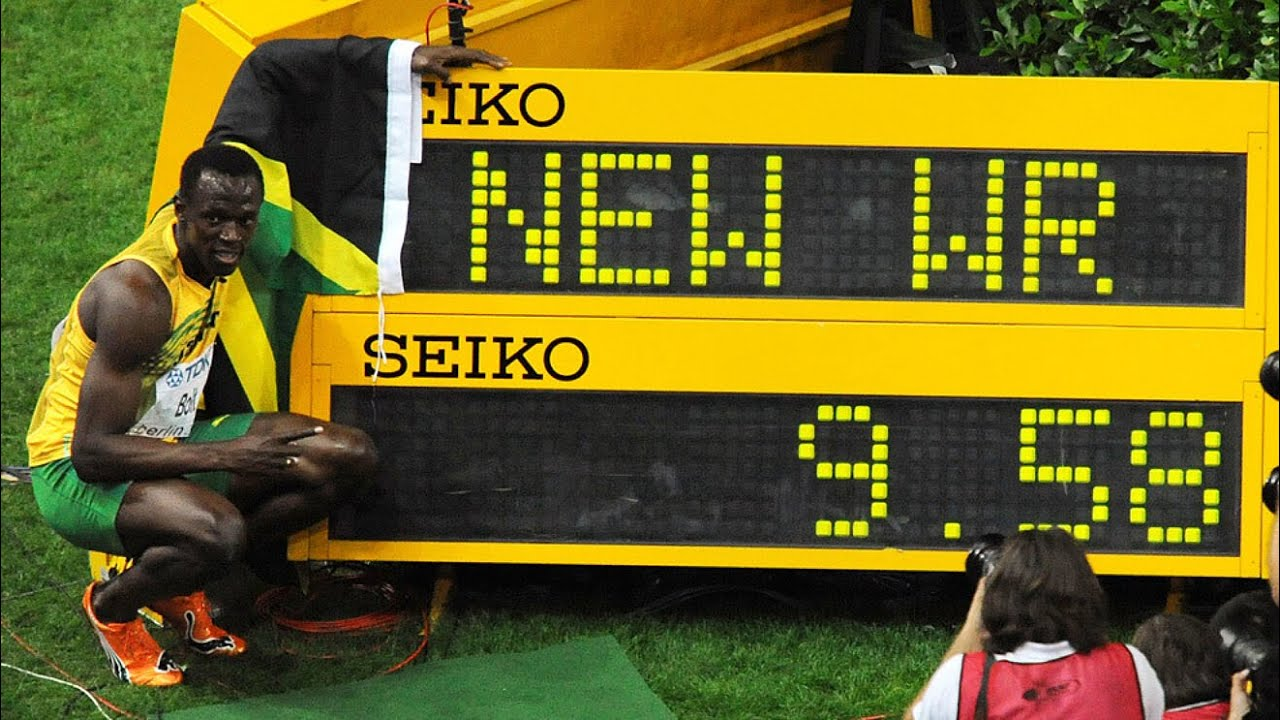
\includegraphics[scale=0.08]{figs/D10-CK1-001-5}}
	\choiceTF[t]
	{Chuyển động của Usain Bolt là chuyển động thẳng nhanh dần đều}
	{\True Tốc độ của Usain Bolt khi về đến đích xấp xỉ $\SI{12.38}{\meter/\second}$}
	{Gia tốc trong giai đoạn tăng tốc của Usain Bolt là khoảng $\SI{6}{\meter/\second^2}$}
	{\True Usain Bolt đã duy trì tốc độ tối đa của mình trên đoạn đường dài $\SI{81.46}{\meter}$}
	\loigiai{}
\end{ex}
% ===================================================================
\begin{ex}
\immini{Một vật nhỏ có khối lượng $\SI{5.0}{\kilogram}$ được kéo bằng sợi dây trên sàn nằm ngang. Sợi dây nhẹ, không dãn và làm góc $\SI{25}{\degree}$ so với phương ngang. Hệ số ma sát trượt giữa vật và mặt sàn là $0,15$. Lực kéo tác dụng lên dây có độ lớn $F=\SI{12}{\newton}$. Lấy $g=\SI{9.8}{\meter/\second^2}$.}
{\begin{tikzpicture}
		\coordinate (O) at (0,0);
		\coordinate (A) at ($(O)+(2.5,0)$);
		\coordinate (B) at ($(O)+(25:2)$);
		\filldraw[color=orange!80!brown] (-0.5,-0.25) rectangle (0.5,0.25);
		\draw[line width=6pt, color=gray] (-2.5,-0.36)--(2.5,-0.36);
		\draw[-stealth, blue, line width=1.5pt] (O)--(B);
		\draw[dashed, line width=1pt] (O)--(A);
		\tkzMarkAngle[size=0.75cm,color=red, line width=1.2pt](A,O,B);
		\tkzLabelAngle[color=black,pos=1.2](A,O,B){$\SI{25}{\degree}$};
		\node[above, blue]at(B) {$\vec{F}$};
\end{tikzpicture}}
	\choiceTF[t]
	{Phản lực của mặt sàn tác dụng lên vật bằng $\SI{49}{\newton}$}
	{\True Lực ma sát trượt tác dụng lên vật có độ lớn xấp xỉ $\SI{6.6}{\newton}$}
	{Gia tốc của vật xấp xỉ $\SI{1.08}{\meter/\second^2}$}
	{Người ta tăng dần lực kéo $F$, ngay khi lực kéo có độ lớn $\SI{49}{\newton}$ thì vật bị nâng khỏi mặt sàn}
	\loigiai{}
\end{ex}
\Closesolutionfile{ans}
\section{Câu trắc nghiệm trả lời ngắn} \textit{Thí sinh trả lời từ câu 1 đến câu 6}
\setcounter{ex}{0}
\Opensolutionfile{ans}[ans/D10-CK1-001-TL]
% ===============================================================
\begin{ex}
	Một chất điểm chuyển động thẳng có phương trình vận tốc theo thời gian dạng $v=15-3t$, trong đó $t$ tính bằng giây và $v$ tính bằng $\si{\meter/\second}$. Tính tốc độ trung bình của chất điểm trong khoảng thời gian từ $t_1=\SI{0}{\second}$ đến $t_2=\SI{2}{\second}$ theo đơn vị mét/giây $\left(\si{\meter/\second}\right)$.
	\shortans[oly]{12}
	\loigiai{
		
	}
\end{ex}
% ===============================================================
\begin{ex}
	Một vật khối lượng $m=\SI{1.5}{\kilogram}$ bắt đầu chuyển động nhanh dần đều trên mặt phẳng ngang dưới tác dụng của lực kéo theo phương ngang, độ lớn $F_{\mathrm{k}}=\SI{7.5}{\newton}$. Hệ số ma sát giữa vật và mặt phẳng ngang là $\mu=0,2$. Lấy $g=\SI{10}{\meter/\second^2}$. Tính gia tốc của vật theo đơn vị $\si{\meter/\second^2}$.
	\shortans[oly]{3}
	\loigiai{
		
	}
\end{ex}
% ===============================================================
\begin{ex}
\immini{Một vòng đệm bằng đồng có đường kính ngoài và đường kính trong lần lượt là $\SI{4.50}{\centi\meter}$ và $\SI{1.25}{\centi\meter}$. Bề dày của vòng đệm là $\SI{1.50}{\milli\meter}$. Đồng có khối lượng riêng là $\SI{8600}{\kilogram/\meter^3}$. Lấy gia tốc trọng trường $g=\SI{9.8}{\meter/\second^2}$, $\pi=3,14$. Trọng lượng của vòng đệm trên là bao nhiêu newton $\left(\si{\newton}\right)$? \textit{(Kết quả làm tròn đến chữ số hàng phần mười)}.}
{
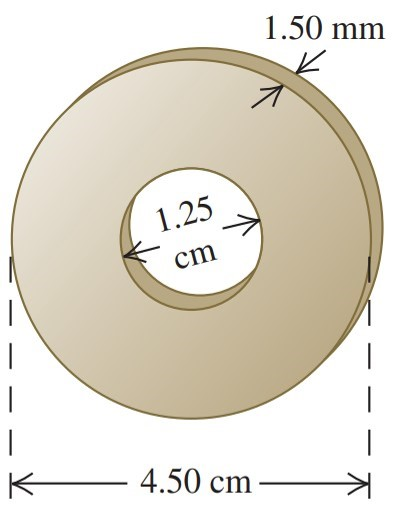
\includegraphics[scale=0.4]{figs/D10-CK1-001-3}
}
	\shortans[oly]{0,2}
	\loigiai{
		
	}
\end{ex}

% ===============================================================
\begin{ex}
	\immini{Một khối hộp có dạng hình lập phương nặng $\SI{1}{\kilogram}$  đặt trong nước nguyên chất có khối lượng riêng $\rho=\SI{1000}{\kilogram/\meter^3}$. Mỗi cạnh của khối hộp có độ dài $\SI{10}{\centi\meter}$. Cho $g=\SI{10}{\meter/\second^2}$. Tính lực đẩy Archimedes tác dụng lên khối hộp nếu nó được nhúng hoàn toàn trong nước. \textit{(Kết quả tính theo đơn vị newton $\left(\si{\newton}\right)$)}.}
	{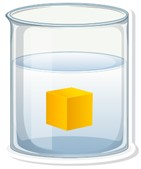
\includegraphics[scale=0.4]{figs/D10-CK1-001-1}}
	\shortans[oly]{10}
	\loigiai{
		
	}
\end{ex}
% ===============================================================
\begin{ex}
	\immini{Một cơ hệ bố trí như hình bên được sử dụng trong bệnh viện để hỗ trợ tác dụng lực kéo ngang lên chân bị thương của bệnh nhân. Lấy gia tốc trọng trường $g=\SI{9.8}{\meter/\second^2}$. Tính độ lớn hợp lực kéo ngang tác dụng lên giá đỡ bàn chân theo đơn vị newton $\left(\si{\newton}\right)$. \textit{(Kết quả làm tròn đến chữ số hàng đơn vị)}.}{
		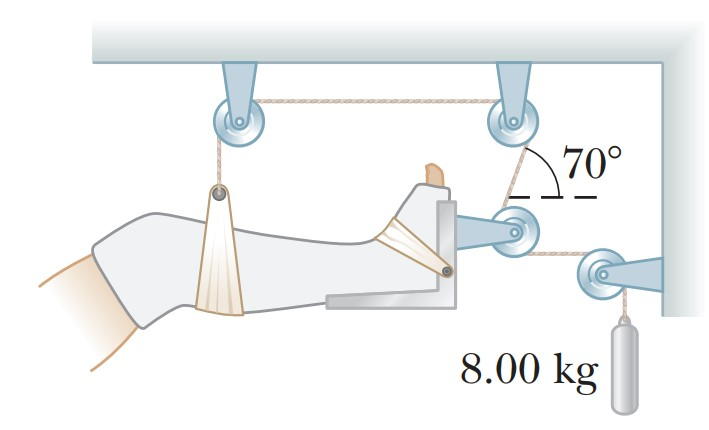
\includegraphics[scale=0.35]{figs/D10-CK1-001-6}
	}
	\shortans[oly]{105}
	\loigiai{
		
	}
\end{ex}
% ===============================================================
\begin{ex}
\immini{Một vật khối lượng $m=\SI{1}{\kilogram}$ có thể trượt trên mặt phẳng nghiêng góc $\alpha=\SI{30}{\degree}$ so với mặt ngang. Hệ số ma sát giữa vật và mặt phẳng nghiêng là $\mu=0,2$. Lực $\vec{F}$  không đổi tác dụng vào vật có phương nằm ngang (hình vẽ). Lấy $g=\SI{10}{\meter/\second^2}$.	Xác định độ lớn của lực $\vec{F}$ để vật trượt đều lên mặt phẳng nghiêng. \textit{(Kết quả tính theo đơn vị $\si{\newton}$ và làm tròn đến chữ số hàng phần mười)}.
}
{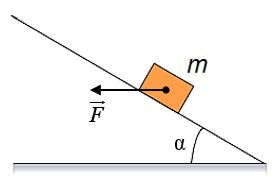
\includegraphics[scale=0.8]{figs/D10-CK1-001-2}}
	\shortans[oly]{ 8,8}
	\loigiai{
		
	}
\end{ex}
\Closesolutionfile{ans}
\begin{center}
	\textbf{--- HẾT ---}
\end{center}